\section{液压机}\label{sec:5-4}

\begin{wrapfigure}[7]{r}{4cm}
    \centering
    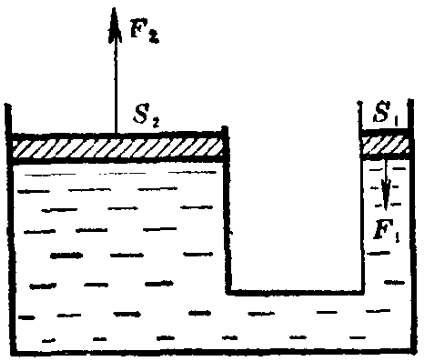
\includegraphics[width=3.5cm]{../pic/czwl1-ch5-9a}
    \caption{液压机原图}\label{fig:5-9}
\end{wrapfigure}

帕斯卡定律在生产技术中有很重要的应用。能够举起重物的油压千斤顶,锻压钢铁的水压机,
榨油用的榨油机等,都是利用帕斯卡定律工作的。这一类机械统称为液压机。

图 \ref{fig:5-9} 是液压机的原理图。它有两个大小不同的液缸,液缸里充满水或油,充水的叫做水压机,充油的叫做油压机。
两个液缸里都有活塞。在小活塞上加压力的时候,小活塞对液体的压强就通过液体传递给大活塞,把大活塞压上去。

使用液压机有什么好处呢?现在我们来研究这个问题。假设小活塞的横截面积是 $S_1$,
加在小活塞上的向下的压力是 $F_1$,那么小活塞对液体的压强 $p = \dfrac{F_1}{S_1}$。
\CJKunderwave{根据帕斯卡定律,这个压强将被液体大小不变地传递给大活塞,所以大活塞受到的压强也等于\,$p$\,}。
如果大活塞的横截面积是 $S_2$,那么压强 $p$ 在大活塞上产生的向上的压力 $F_2 = p\,S_2$。
把 $p = \dfrac{F_1}{S_1}$  代入前面的式子,可得 $F_2 = \dfrac{F_1}{S_1} S_2$,或写作
$$ \dfrac{F_2}{F_1} = \dfrac{S_2}{S_1} \;\juhao $$

上式左边的 $\dfrac{F_2}{F_1}$ 表示大活塞上的压力是小活塞上的压力的多少倍,
右边的 $\dfrac{S_2}{S_1}$ 表示大活塞的横截面积是小活塞的横截面积的多少倍。
从上式可以看出,
\CJKunderwave{大活塞的横截面积是小活塞横截面积的多少倍,在大活塞上得到的压力就是加在小活塞上的压力的多少倍}。
因此,在小活塞上加不大的压力,在大活塞上就可以得到很大的压力。这就是使用液压机的好处。

\begin{figure}[htbp]
    \centering
    \begin{minipage}{7cm}
    \centering
    \vspace{17em}
    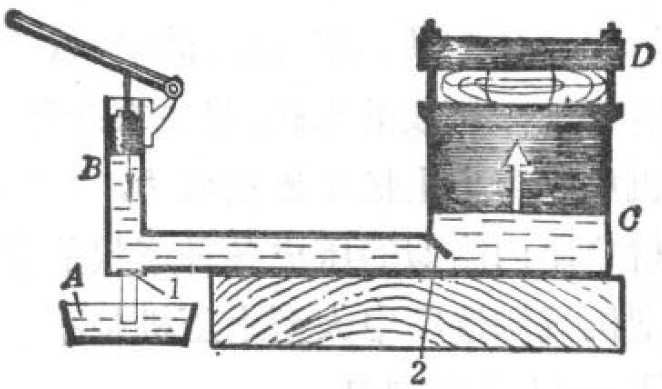
\includegraphics[width=7cm]{../pic/czwl1-ch5-10}
    \caption{液压机的构造}\label{fig:5-10}
    \end{minipage}
    \qquad
    \begin{minipage}{8cm}
    \centering
    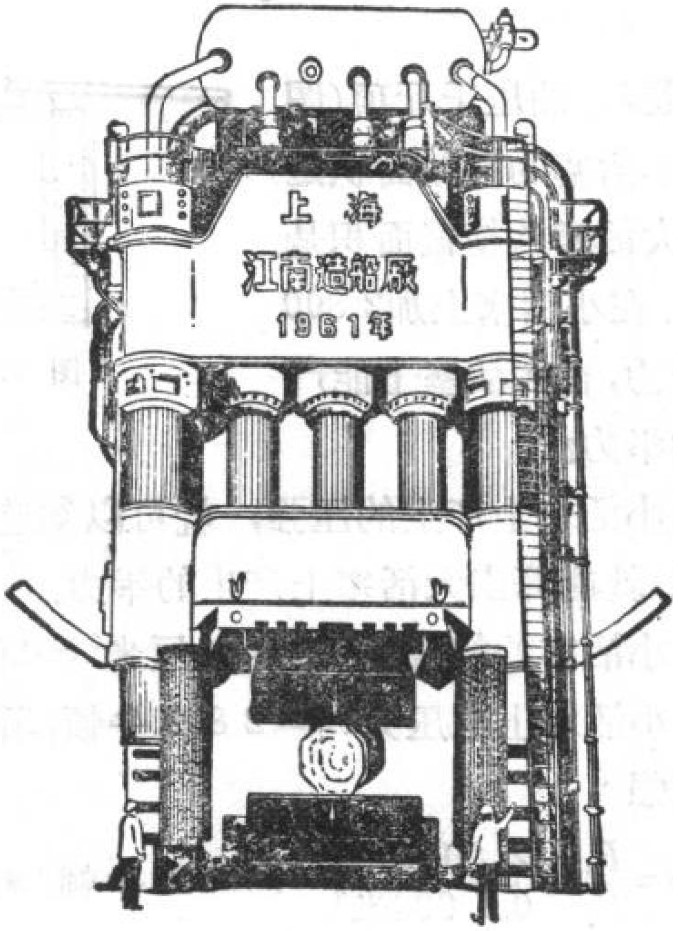
\includegraphics[width=8cm]{../pic/czwl1-ch5-11}
    \caption{万吨水压机}\label{fig:5-11}
    \end{minipage}
\end{figure}


图 \ref{fig:5-9} 只表示液压机的原理。实际的液压机,为了能够连续工作,还要添加必要的零件,它的构造如图 \ref{fig:5-10} 所示。
液压机的工作过程如下:提起小活塞时,容器 $A$ 里的液体就推开阀门 $1$ 进入小液缸 $B$ 中。
压下小活塞时,阀门 $1$ 关闭,小液缸中的液体就在压力的作用下推开阀门 $2$ 进入大液缸 $C$ 中,推着大活塞上升。
反复提压小活塞,就能够把液体不断压入大液缸中,使大活塞逐渐上升。被压榨物体放在大活塞上,
当大活塞上升到使物体顶着上面固定不动的上平台 $D$ 时,物体就被挤压。

液压机可以用来压制胶合板,提举重物,榨油。大的液压机可以锻压钢铁,经过锻压的钢铁内部变得密实、均匀、有韧性。
制成的车轴、机车车轮等不易断裂。万吨水压机可以产生上亿牛顿的压力,能够把几百吨的大型钢材象揉面团似的压成各种形状的钢件。
在造船厂,重型机械制造厂中大型水压机是不可缺少的重要设备。图 \ref{fig:5-11} 是我国自己设计制造的第一台万吨水压机。

\liti 油压千斤顶(图 \ref{fig:5-12})的小活塞的横截面积是 $4 \pflm$,大活塞的横截面积是 $112 \pflm$。
在小活塞上加 2\;800 牛顿的压力,在大活塞上能产生多大的举力?

求出小活塞上产生的压强,就可以知道大活塞受到的压强,就能算出大活塞上产生的举力。

解:小活塞的横截面积 $S_1 = 4 \pflm = 0.0\, 004 \pfm$。

\begin{wrapfigure}[12]{r}{4cm}
    \centering
    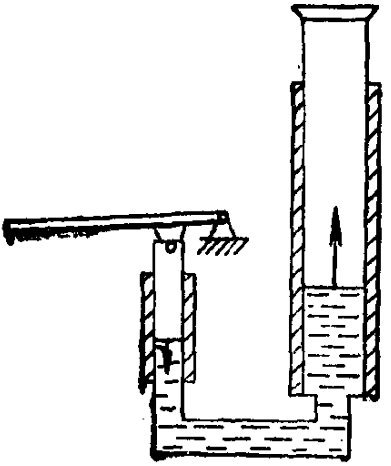
\includegraphics[width=3.5cm]{../pic/czwl1-ch5-12}
    \caption{液压机原图}\label{fig:5-12}
\end{wrapfigure}

加在小活塞上的压力 $F_1 = 2\;800 \niudun$,所以小活塞对油的压强
$$ p = \dfrac{F_1}{S_1} = \dfrac{2\;800 \niudun}{0.0\;004 \pfm} = 7 \times 10^6 \ndmpfm \;\juhao $$

根据帕斯卡定律,大活塞受到的压强也等于 $p$,大活塞的横截面积 $S_2 = 112 \pflm = 0.0\;112 \pfm$,
所以大活塞上产生的举力
$$ F_2 = p\,S_2 = 7 \times 10^6 \ndmpfm \times 0.0\;112 \pfm = 7.84 \times 10^4 \niudun \;\juhao $$

答:大活塞上产生的举力是 $7.84 \times 10^4$ 牛顿。

这道题也可以用别的方法来解。
譬如,先求出大活塞的横截面积是小活塞的几倍,用求得的倍数乘以小活塞上的压力,就得出大活塞产生的举力。
又譬如,根据公式 $\dfrac{F_2}{F_1} = \dfrac{S_2}{S_1}$,得出 $F_2 = \dfrac{S_2}{S_1} \; F_1$,
把题中给出的数据代入,即可求出大活塞产生的举力。
实际上,不少物理问题都是有多种解答方法的。
经常注意这一点,在解答过一个物理问题后,再想想还有没有别的解法,对提高我们灵活运用物理知识的能力是很有好处的。


\lianxi

(1) 在一个塑料袋里装上水,用线把口扎紧,再用针在袋上穿几个小孔,用力捏袋上任何地方,水都从小孔喷射出来(图 \ref{fig:5-13})。为什么?

\begin{figure}[htbp]
    \centering
    \begin{minipage}{4cm}
    \centering
    \vspace{8em}
    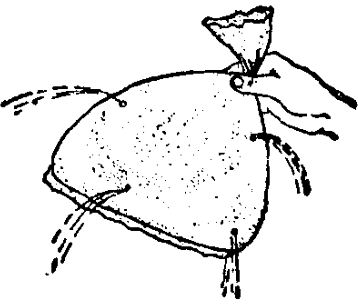
\includegraphics[width=4cm]{../pic/czwl1-ch5-13}
    \caption{}\label{fig:5-13}
    \end{minipage}
    \qquad
    \begin{minipage}{10cm}
    \centering
    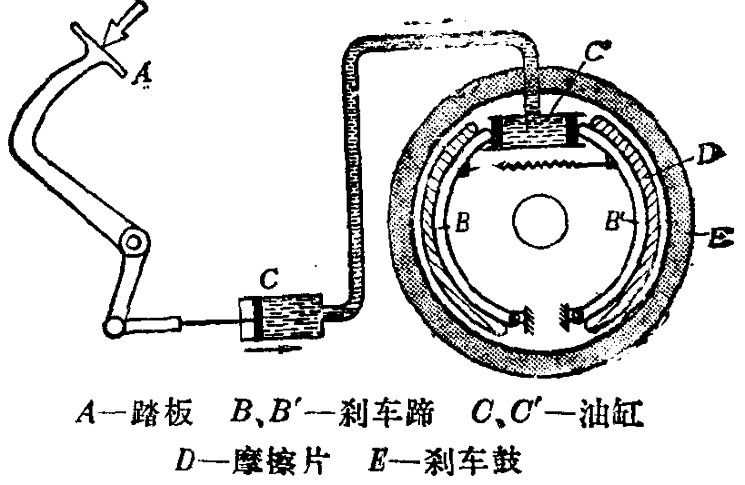
\includegraphics[width=10cm]{../pic/czwl1-ch5-14}
    \caption{}\label{fig:5-14}
    \end{minipage}
\end{figure}

(2) 图 \ref{fig:5-14} 是汽车的液压传动刹车示意图(只画出一个车轮)。用脚往下踩刹车踏板 $A$ 时,刹车蹄 $B$、$B'$ 就张开,
把摩擦片 $D$ 紧压在刹车鼓 $E$ 上,使车轮停止转动。刹车蹄 $B$、$B'$ 为什么能张开?

(3) 在图 \ref{fig:5-10} 所示的液压机中,小活塞每压下一次通过的距离和大活塞升高的距离哪个大?
由此看出液压机虽然增大了力,却多用了什么?

(4) 有一台水压机,小活塞的横截面积是 $4 \pflm$,大活塞的横截面积是 $120 \pflm$。
在小活塞上加 160 牛顿的压力,在大活塞上能够产生多大的力?

(5) 有一台水压机,在小活塞上加 $2 \times 10^5$ 帕斯卡的压强时,大活塞上能产生 $3 \times 10^5$ 牛顿的压力,
大活塞的面积是多大?

